\section{Introduction}
In the beginning, there was FORTRAN.

\section{Introduction to Teams}\label{sec:teams}
The existing coarray definition in Fortran 2008 does not provide for an environment
where a subset of the images can easily work on part of an application without affecting
other images in the program.  Grouping the images of a program into nonoverlapping
teams allows one to execute more effectively and independently parts of a larger
problem.  A class of problems that can benefit from this feature is multiphysics codes
(e.g.  climate models).
Such feature, called \textit{Teams} in the Fortran 2015 standard, can significantly reduce the amount of off-node
communication on an exascale machine, in particular when an entire team of images
fits within a single compute node.
So far, the only compiler with a partial support for this new feature is the GNU Fortran Compiler (from now on
called GFortran) and a special version of the OpenCoarrays library.
In this Section we are going to introduce the basic constructs of \textit{Teams} and how OpenCoarrays implements them.

A team of images is a set of images that can readily execute independently of other images.
Initially, the current team consists of all images and this is
known as the initial team. Except for the initial team, every team has a unique parent team. A team is divided
into new teams by executing a \texttt{FORM TEAM} statement.
Each new team is identified by an integer value known
as its team number. Information about the team to which the current image belongs can be determined by the
processor from the collective value of the team variables on the images of the team.

During execution, each image has a current team, which is only changed by execution of \texttt{CHANGE TEAM} and
\texttt{END TEAM} statements. Executing a \texttt{CHANGE TEAM} statement changes the current team to the team specified
by the team-variable, and execution of the corresponding \texttt{END TEAM} statement restores the current team back
to that immediately prior to execution of the \texttt{CHANGE TEAM} statement.

\subsection{Teams implementation}\label{subsec:teams_implementation}

From an MPI prospective, a Fortran team is comparable to an MPI communicator. The \texttt{FORM TEAM} statement can be
implemented using \texttt{MPI\_Comm\_split} and 



\begin{figure*}
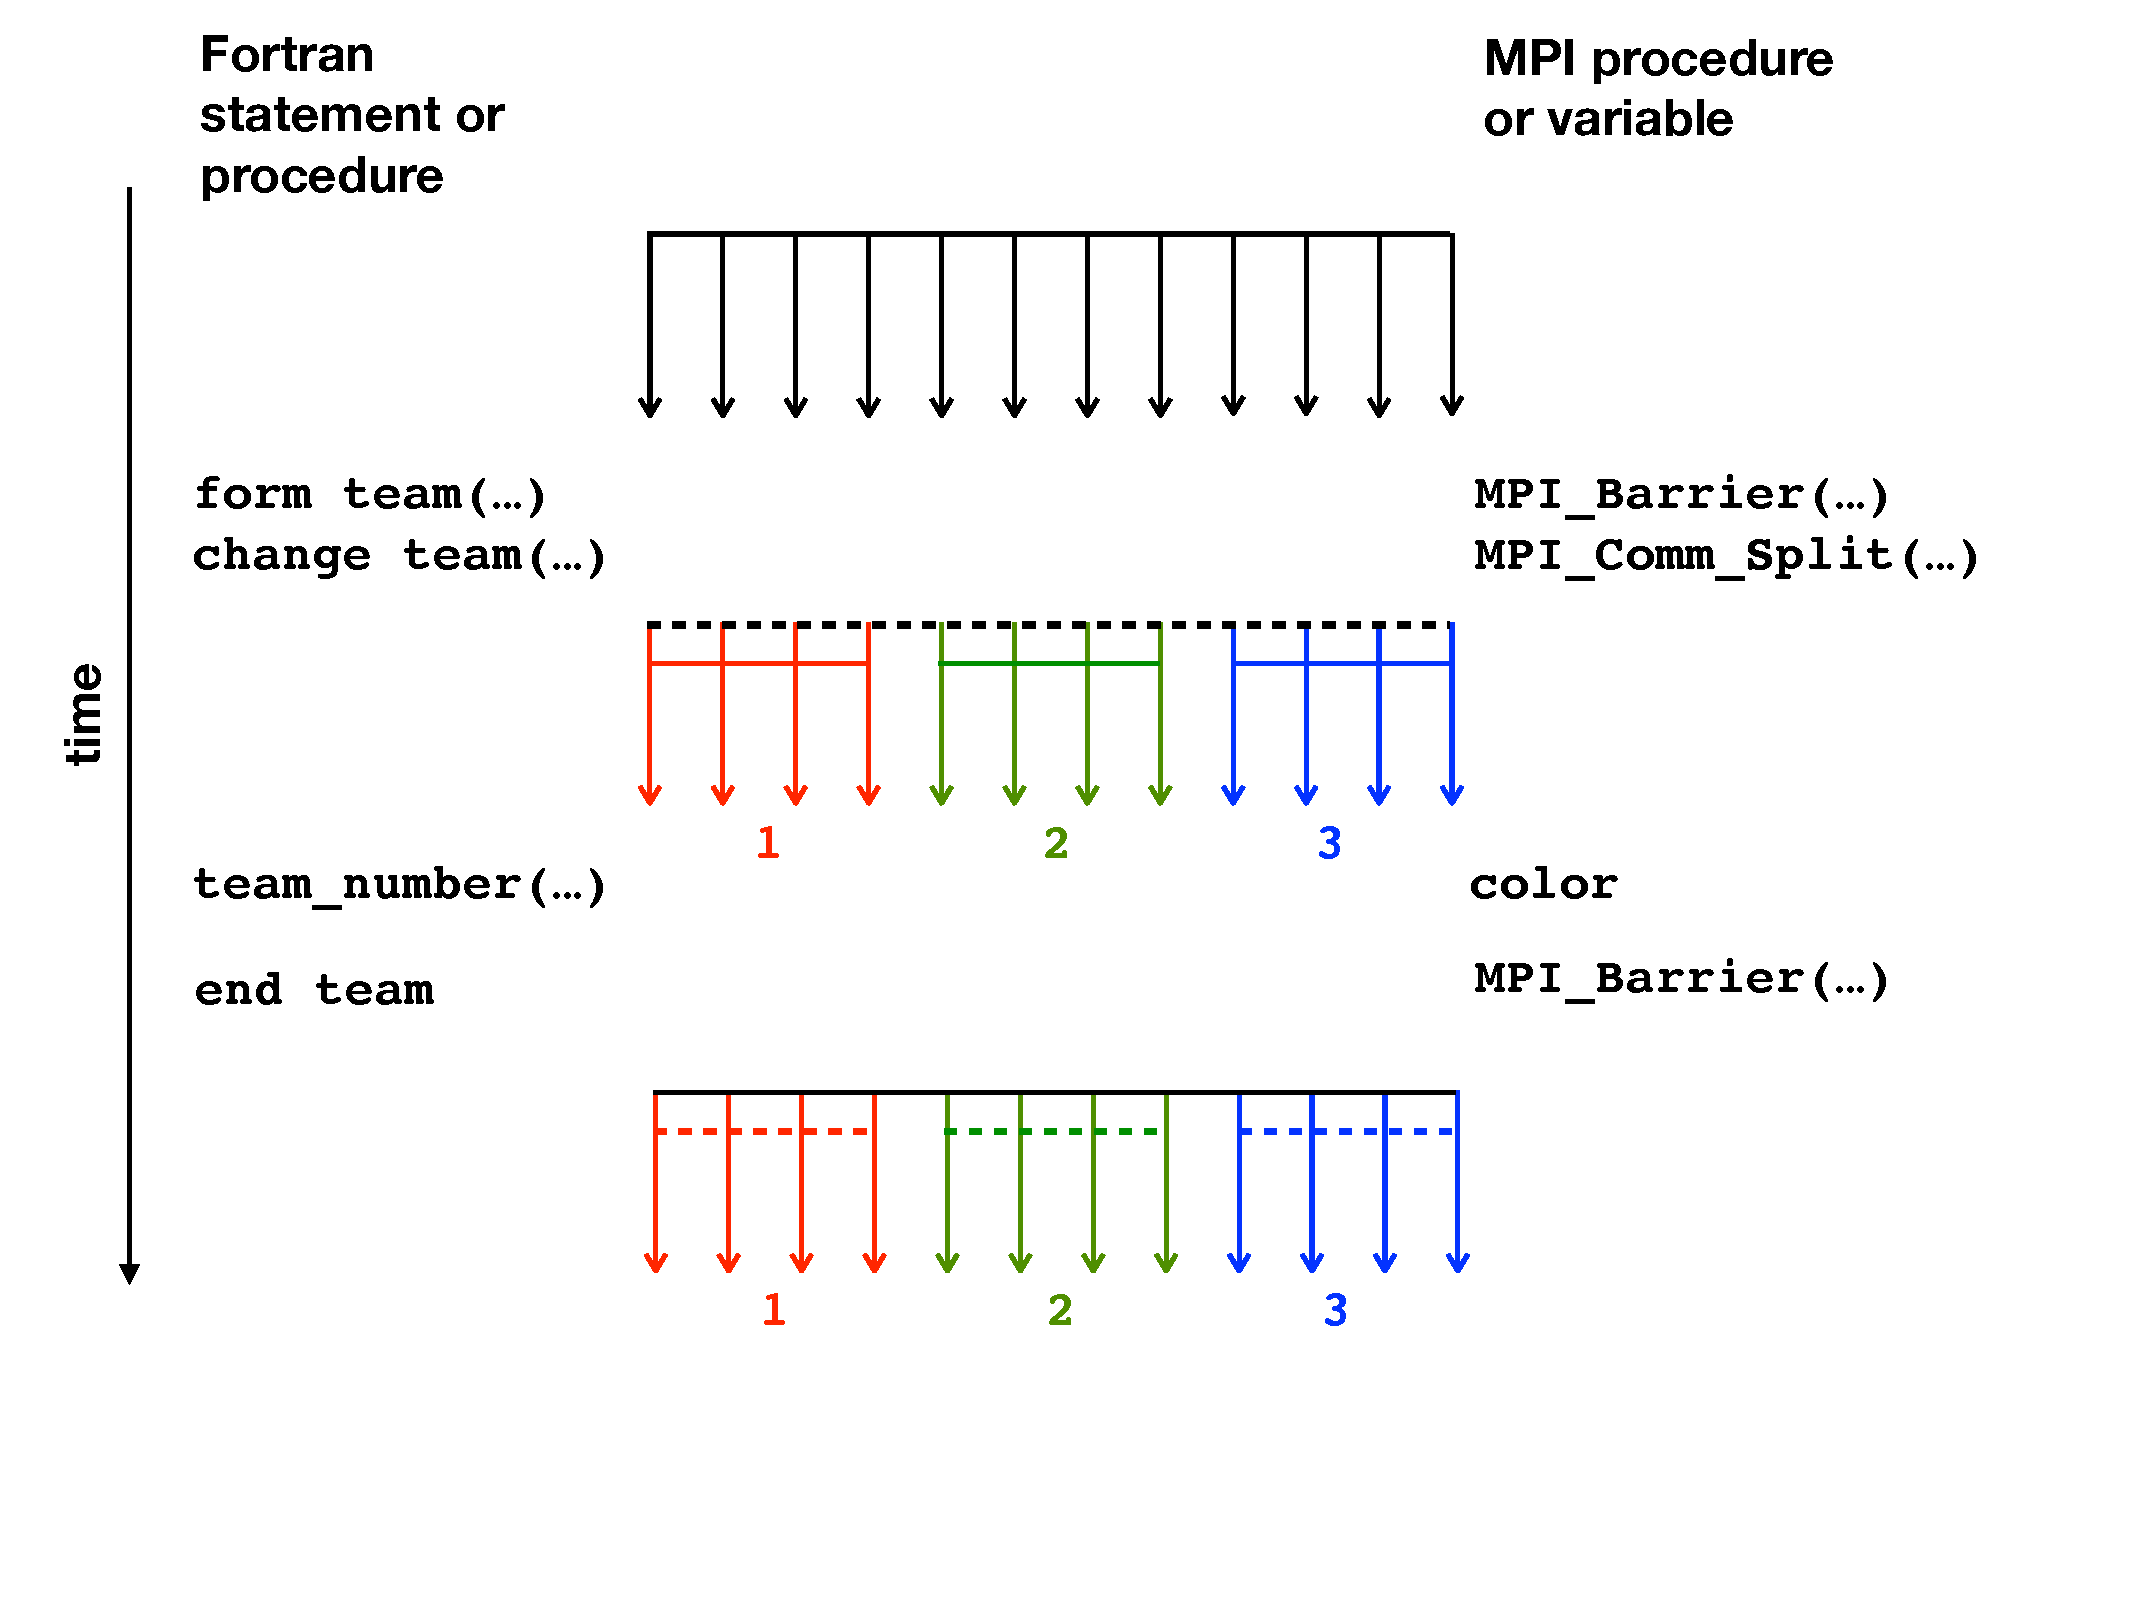
\includegraphics[width=0.7\textwidth]{figures/teams}
\vspace{-36pt}
\caption{Schematic depiction of a Fortran program executing over time (left axis) in 12 images (top) thatcommunicate with each other through global means (black horizontal bar) and later communicating within subgroups (colored horizontal bars).  Horizontal lines represent the communication mechanisms (default=solid, optional=dashed).  Fortran concepts or on the left.  The underlying \gls{mpi} concepts are the right.}
\end{figure*}
%

\begin{figure*}
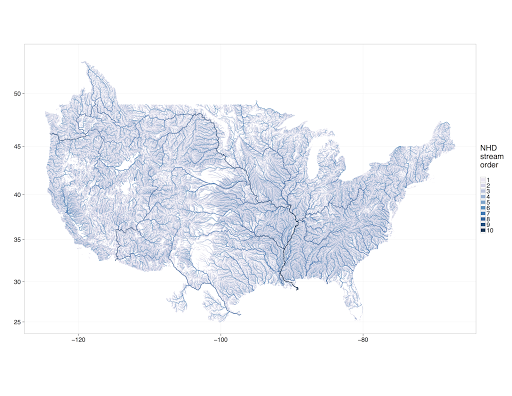
\includegraphics[width=0.7\textwidth]{figures/hydro-map}
\vspace{-36pt}
\caption{Sample WRF-Hydro simulation domain.}
\end{figure*}
%

%%%
%%% Sample tables
%%%

%\begin{table}
%  \caption{Frequency of Special Characters}
%  \label{tab:freq}
%  \begin{tabular}{ccl}
%    \toprule
%    Non-English or Math&Frequency&Comments\\
%    \midrule
%    \O & 1 in 1,000& For Swedish names\\
%    $\pi$ & 1 in 5& Common in math\\
%    \$ & 4 in 5 & Used in business\\
%    $\Psi^2_1$ & 1 in 40,000& Unexplained usage\\
%  \bottomrule
%\end{tabular}
%\end{table}

%\begin{table*}
%  \caption{Some Typical Commands}
%  \label{tab:commands}
%  \begin{tabular}{ccl}
%    \toprule
%    Command &A Number & Comments\\
%    \midrule
%    \texttt{{\char'134}author} & 100& Author \\
%    \texttt{{\char'134}table}& 300 & For tables\\
%    \texttt{{\char'134}table*}& 400& For wider tables\\
%    \bottomrule
%  \end{tabular}
%\end{table*}
% end the environment with {table*}, NOTE not {table}!

%It is strongly recommended to use the package booktabs~\cite{Fear05}
%and follow its main principles of typography with respect to tables:
%\begin{enumerate}
%\item Never, ever use vertical rules.
%\item Never use double rules.
%\end{enumerate}
%It is also a good idea not to overuse horizontal rules.


%%%
%%% Sample figures
%%%

%\begin{figure}
%\includegraphics{fly}
%\caption{A sample black and white graphic.}
%\end{figure}

%\begin{figure}
%\includegraphics[height=1in, width=1in]{fly}
%\caption{A sample black and white graphic
%that has been resized with the \texttt{includegraphics} command.}
%\end{figure}

%\begin{figure*}
%\includegraphics{flies}
%\caption{A sample black and white graphic
%that needs to span two columns of text.}
%\end{figure*}
%
%\begin{figure}
%\includegraphics[height=1in, width=1in]{rosette}
%\caption{A sample black and white graphic that has
%been resized with the \texttt{includegraphics} command.}
%\end{figure}

%\end{document}  % This is where a 'short' article might terminate



\appendix
%Appendix A
\section{Code listing}
% This next section command marks the start of
% Appendix B, and does not continue the present hierarchy
\section{Anything else?}

\begin{acks}
  The authors would like to thank the CISL and RAL Visitor Program

  The work is
  supported by the \grantsponsor{GSxxxxx}{National
  Science Foundation China}{http://dx.doi.org/zz.yyyyy/xxxxx} under Grant
  No.:~\grantnum{GSxxxxx}{yyyyyyy}

\end{acks}
